%%%%%%%%%%%%%%%%%%%%%%%%%%%%%%%%%%%%%%%%%
% Dmitry Khodakov CV.
%%%%%%%%%%%%%%%%%%%%%%%%%%%%%%%%%%%%%%%%%

\documentclass[a4paper, oneside, final]{scrartcl}
\usepackage{scrpage2} % Provides headers and footers configuration
\usepackage{titlesec} % Allows creating custom \section's
\usepackage{marvosym} % Allows the use of symbols
\usepackage{tabularx,colortbl} % Advanced table configurations
\usepackage{fontspec} % Allows font customization
\usepackage{color}
\usepackage[usenames,dvipsnames]{xcolor}

\usepackage{polyglossia}
\setmainlanguage{russian} 
\setotherlanguage{english}
\newfontfamily\russianfont[Script=Cyrillic]{Tahoma}

\defaultfontfeatures{Mapping=tex-text}

\titleformat{\section}{\color{BrickRed}\large\scshape\raggedright}{}{0cm}{}[\titlerule] % Section formatting

%\titleformat{name=\section}[block]
%  {\color{BrickRed}\large\scshape\raggedright}
%  {}
%  {0pt}
%  {\colorsection}
%  [\titlerule]
%\titlespacing*{\section}{0pt}{\baselineskip}{\baselineskip}

\newcommand{\colorsection}[1]{%
  \colorbox{gray!15}{\parbox{\dimexpr\textwidth-2\fboxsep}{\thesection\ #1}}}
\pagestyle{scrheadings} % Print the headers and footers on all pages
\addtolength{\voffset}{-2.3cm} % Adjust the vertical offset - less whitespace at the top of the page
\addtolength{\textheight}{5.7cm} % Adjust the text height - less whitespace at the bottom of the page

% FOOTER SECTION
%----------------------------------------------------------------------------------------

\renewcommand{\headfont}{\normalfont\rmfamily\scshape} % Font settings for footer

\cofoot{
\addfontfeature{LetterSpace=10.0}\fontsize{12.5}{12}\selectfont % Letter spacing and font size
{\Letter} dmitryhd@gmail.com \ {\Large\Telefon} (915) 219-219-8 % Your email address and phone number % TODO: fake number
}
\newcommand{\tabitem}{{\textbullet}~~}

\usepackage{graphicx}
\graphicspath{ {/} }
%----------------------------------------------------------------------------------------

\begin{document}

\begin{center} % Center everything in the document

% HEADER SECTION
%----------------------------------------------------------------------------------------

\begin{tabularx}{0.99\linewidth}{m{10cm}m{4cm}}

{\addfontfeature{LetterSpace=5.0}\fontsize{24}{24}\selectfont\scshape Dmitriy Khodakov} & % Your name at the top 
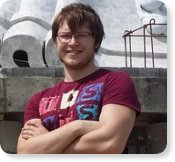
\includegraphics[width=4cm]{dim-av.png} \\
\end{tabularx}

\section{\textbf{Education}}

\begin{tabularx}{0.99\linewidth}{p{2cm}p{11.8cm}}
\multicolumn{2}{l}{\textbf{Moscow Institute of Physics and Technology (State University) (MIPT)}} \\
&\quad\\
 2012 - 2014 &  {Master's Degree: Machine Learning and Neural Networks} \\
 2008 - 2012 &  {Bachelor's Degree: Computer Systems Networking and Telecommunications}
    \newline Base organisation: Institute for Information Transmission Problems (IITP RAS) \\
\end{tabularx}

\section{\textbf{Experience}}
\begin{tabularx}{0.99\linewidth}{p{2cm}p{11.8cm}}

\multicolumn{2}{l}{\textbf{Orion - \textit{Lead Software Developer - Python}}} \\
03.2013 Present \rule{1.9cm}{.1pt} 2 years \newline 2 months &
    \tabitem Development of software monitoring and management system \newline
    \tabitem GPU cluster (Linux, Windows) \newline
    \tabitem Back-end on Python, data collection by SNMP/IPMI protocols \newline
    \tabitem MySQL database engine \newline
    \tabitem Web based GUI (Django with JavaScript/jQuery front-end)\newline
    \tabitem Gui migrated to Flask\newline
    \tabitem TODO: write about deployment, RHEL, hardware \\ 
& ~ \\
\multicolumn{2}{l}{\textbf{Telum - Researcher/Software Engineer - C++}} \\
 08.2011 03.2013 \rule{1.9cm}{.1pt} 1 year \newline 7 months &
    \tabitem Implementation of custom wireless MAC layer protocol in C++ \newline
    \tabitem Modelling and simulation of this protocol in NS3 \newline
    \tabitem About 200k lines of C++ code \newline
    \tabitem Analysis and implementation of various wireless protocols \newline
    \tabitem Implementation of RSVP and RoHC protocols \newline
    \tabitem Mathematical modelling and data analysis on R language and Python
\\ 
\end{tabularx}

\section{\textbf{Skills}}
\begin{tabularx}{0.99\linewidth}{ p{2cm} p{11.8cm} }
Languages & Python, Javascipt, C++/C, Bash, R \\
Instrumets & Git, SVN, Mercurial, Jira, Redmine, Agile/Scrum, Vim, UML \\
Academic & Theory of telecommunications, Machine learning, Software Architecture \\
Frameworks & Django, JQuery, NS3 \\
Speak & English (technical), Russian (mother language), Spanish (castellano) (basic)  \\
OS & Linux system administration \\
\end{tabularx}

%----------------------------------------------------------------------------------------

\section{\textbf{Certifications}}

\begin{tabularx}{0.99\linewidth}{p{2cm} p{8.8cm} p{2cm}}
2013 & \textbf{Machine Learning by Andrew Ng} & Stanford \\
2014 & \textbf{Statistical Learning} & Stanford  \\
2014 & \textbf{Algorithms: Design and Analysis, Part 1} & Stanford  \\
2014 & \textbf{Algorithms: Design and Analysis, Part 2} & Stanford  \\
\end{tabularx}

%---------------------------------------------------------------------------------

\end{center}

\end{document}
